\documentclass[a4paper, 10pt]{scrartcl}

\usepackage{a4wide}
\usepackage[utf8]{inputenc}
\usepackage[ngerman]{babel}
\usepackage[T1]{fontenc}
\usepackage{amsmath}
\usepackage{graphicx}
\usepackage{listings}
\usepackage{hyperref}

\usepackage{scrpage2}
\pagestyle{scrheadings}
\clearscrheadfoot

\makeatletter



\title{Vim - Introduction}
\author{Lars Hübner}
\date{13. May 2018}

\ihead{Vim - Introduction}
\ifoot{Lars Hübner}
\ofoot{\pagemark}

\begin{document}
\section{Installation}
You can install Vim on Windows from \href{www.vim.org/download.php}{www.vim.org/download.php}.
Just click on - PC: MS-DOS and MS-Windows - and download the latest version of the gvim.exe. This installer sets up everything you need. 
\\
If you have a Linux system then Vim is normally preinstalled. Otherwise you can find also all available downloads on the vim donwload page.
\section{Folder structure}
Windows: Vim Folder

- vim80 (folder containing the executables)

- vimfiles (folder containing all the plugins and addons)

- \_virmc (file containing all the settings and configurations)
\\
\\
Linux:

- .vim (folder containing all the plugins and addons)

- .vimrc (file containing all the settings and configurations)
\section{Concept of modes}
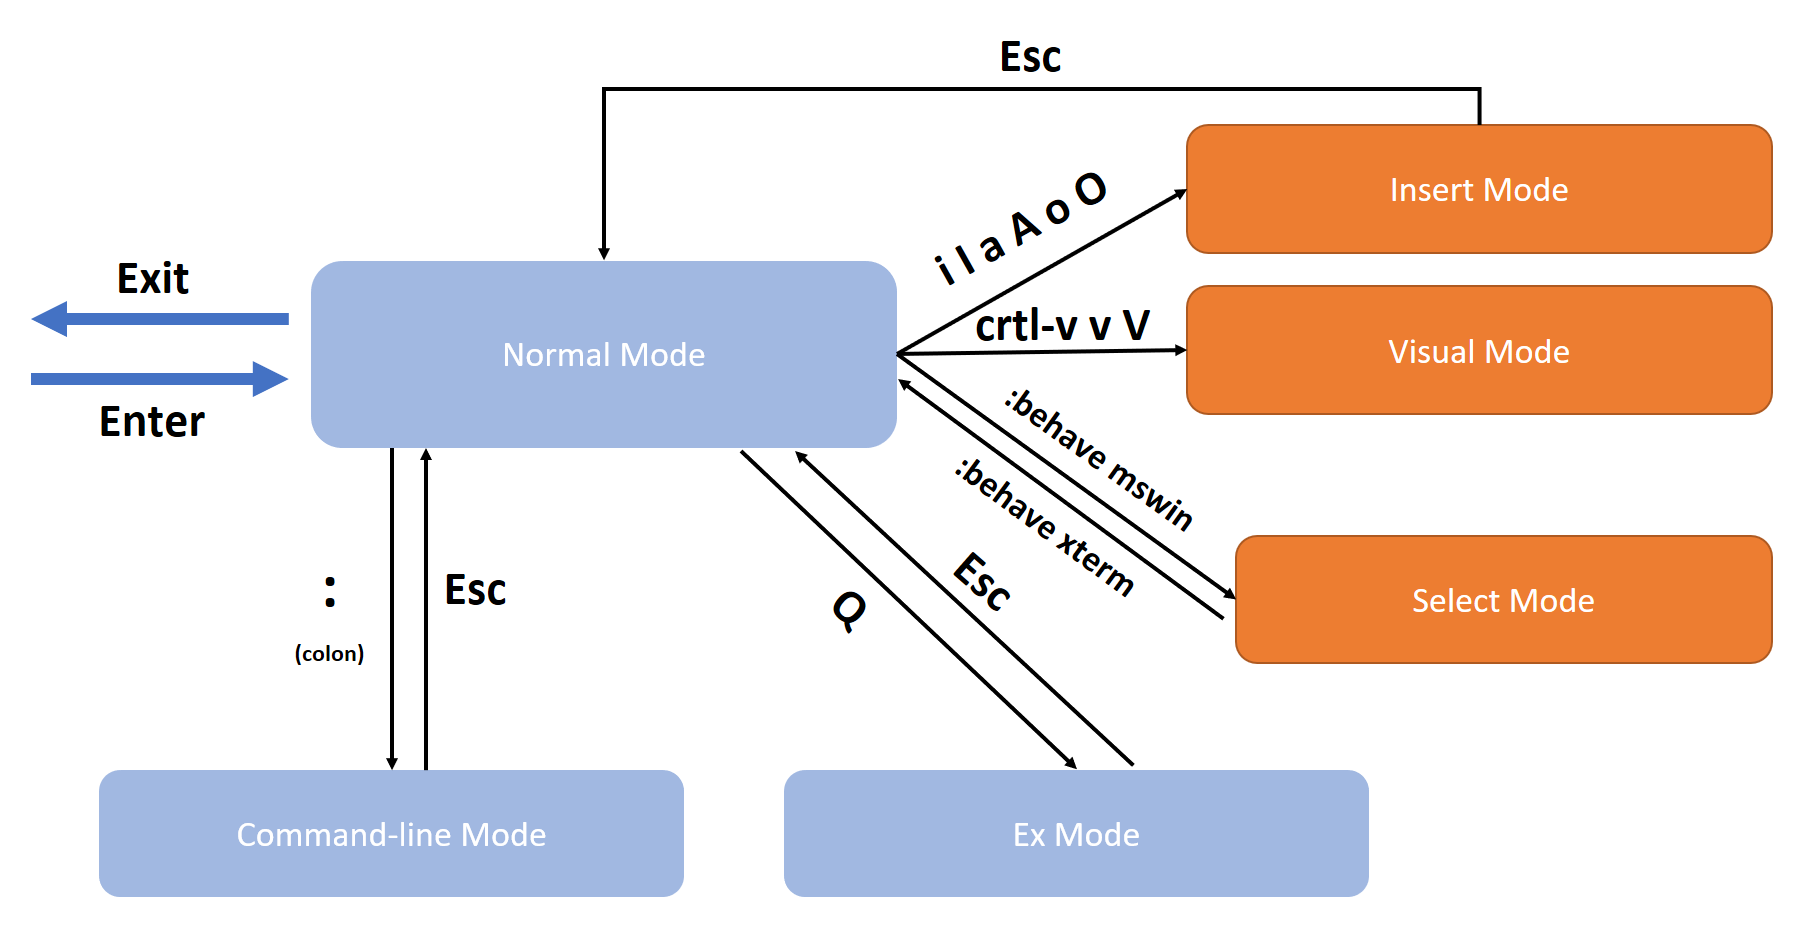
\includegraphics[width=.8\linewidth]{modes.png}
\subsection*{Normal Mode}
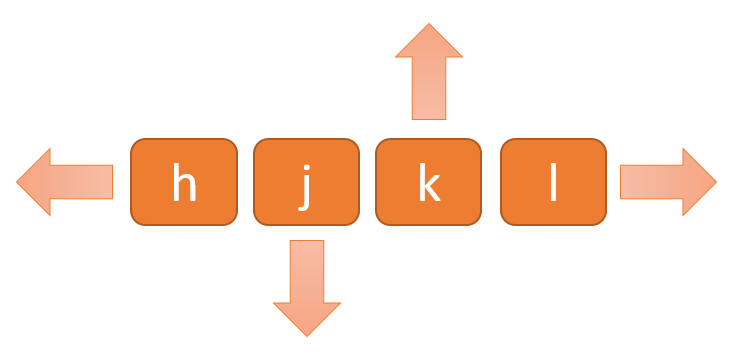
\includegraphics[width=.4\linewidth]{keys.png}
\\
Generalizated action in normal mode: \textbf{[changing-command] [number / option] move-command}
\\
\textbf{Move commands:}

w 	- to the beginning of the next word

e	- to the end of the word

b 	- to the beginning of the previous word

0	- beginning of the Line

\$ 	- end of the Line

1G	- first Line

\#G	- Line Number \#

G	- Last Line
\\
\\
\begin{tabular}{p{7cm} l}
\textbf{Changing commands:} & \textbf{Options:} \\
d  - Delete & i - inner \\
y  - Yank 	& a - all \\
c  - change & \\
\end{tabular}

\section{Made for programmers}
Vim is made from programmers for programmers. It comes with many usefull commands, that can help to manage your code. The following commands are the most important (in my optionion):
\\
\\
\begin{tabular}{l l}
: 5, 10 fo 	& fold from line 5 to 10 \\
za 	& toggle fold \\
>>    << 	& indent line \\
=i\{	& auto indention of the inner braces \{...\} part \\
\%	& jump to corresponding brackets \\
*   oder   \#	& find symbol under curser \\
gd	& goto definition (of variable etc.) \\
/sometext	& search for some Text \\
:\%s/old/new/gc	& replace global in this file with confirmation \\
:find filename	& fuzzy finder for files \\
\end{tabular}
\\
\\
For generating index files of nams in the source code the most common program is \textbf{ctags}\\
 \href{http://ctags.sourceforge.net/}{http://ctags.sourceforge.net/}. This additional program supports about 40 programming languages and the generated tags file can be found by vim. With commands like Ctrl-] you can than goto to a definition of a variable or function and Ctrl-t brings you back to where you come from.
\\
\\
More commands can be found with \textbf{:help} in normal mode. Interesting information about window-management in vim can be found with \textbf{:help window}.
\section{Plugins}
For installing Vim plugins \textit{pathogen} provides a easy and fast way. Simply add the autoload folder of the \href{https://github.com/tpope/vim-pathogen}{vim-pathogen Git Repo} to your vimfiles (.vim) directory and add the lines:
\\
\\
\textbf{execute pathogen\#infect()\\Helptags}
\\
\\
to your vimrc file. All your plugins can be stored (cloned from Git etc.) into a \textbf{bundle} folder that you have to create in the vimefiles (.vim) directory. Now your plugins are going to be included at the vim startup and you have the whole :help support.
\subsection{Useful plugins}
\href{https://github.com/scrooloose/nerdtree}{NERDTree (directory tree) - https://github.com/scrooloose/nerdtree}
\\
\href{https://github.com/tpope/vim-fugitive}{Vim fugitive (Git integration) - https://github.com/tpope/vim-fugitive}
\\
\href{https://github.com/prabirshrestha/vim-lsp}{Vim language server protocol - https://github.com/prabirshrestha/vim-lsp}
\subsection{colors}
\href{https://github.com/flazz/vim-colorschemes}{Vim Colorschemes - https://github.com/flazz/vim-colorschemes}
\\
\\
And set the colors in the vimrc with:

\textbf{colorschemes <name>}
\section{Learn more}
This Handout, the presentation, an example vimrc and more are available in my git repository:
\\
\href{https://github.com/huebnerl/dotfiles/tree/master/e-portfolio}{https://github.com/huebnerl/dotfiles/tree/master/e-portfolio}
\\
There you can also find some example command on how to remap commands and keys in vim.
\\
\\
For learning vim in a deeper way just use the integrated vim tutor:
\\
\textbf{:help tutor}
\end{document}
